\documentclass[12pt,a4paper]{article}
\usepackage[utf8]{inputenc}
\usepackage{amsmath, amssymb, amsthm}
\usepackage{graphicx}
\usepackage{hyperref}
\usepackage{geometry}
\usepackage{listings} % Pentru un afișaj mai bun al codului
\usepackage{xcolor} % Pentru culori în listings

\geometry{margin=2.5cm}

% Configurare pentru listings (opțional, dar arată mai bine)
\lstset{
	language=Python,
	basicstyle=\ttfamily\footnotesize,
	keywordstyle=\color{blue},
	commentstyle=\color{green!40!black},
	stringstyle=\color{purple},
	showstringspaces=false,
	breaklines=true,
	frame=tb, % Doar linii sus și jos pentru un aspect mai curat
	framesep=5pt,
	framexleftmargin=1pt,
	numbers=left,
	numberstyle=\tiny\color{gray},
	tabsize=4,
	captionpos=b % Poziția caption-ului sub listing
}


\title{Sistem de recomandare bazat pe factorizare de matrice și optimizare cu constrângeri}
\author{Gatej Stefan-Alexandru, Potop Horia-Ioan}
\date{\today} % Sau \date{Mai 2024} etc.

\begin{document}

	\maketitle
	\tableofcontents
	\newpage

	\section{Descrierea aplicațiilor}

	Acest sistem de recomandare integrează factorizarea de matrice pentru descoperirea trăsăturilor ascunse ale melodiilor cu aplicații practice de recomandare. Principalul scop este de a oferi sugestii muzicale personalizate.

	Pornind de la o matrice binară (melodie $\times$ tag), aplicăm factorizarea cu constrângeri de non-negativitate pentru a descoperi similarități implicite între melodii. Această bază matematică ne permite să înțelegem mai bine caracteristicile muzicale.

	Pe baza acestor trăsături latente, am dezvoltat două aplicații principale:
	\begin{itemize}
		\item \textbf{Melodie $\rightarrow$ Playlist:} Generează playlisturi noi, coerente, pe baza unei melodii inițiale, respectând constrângeri de durată și non-negativitate.
		\item \textbf{Playlist $\rightarrow$ Melodie:} Identifică melodii noi care completează un playlist existent, folosind centroidul acestuia și optimizare cu penalizări L1/L2.
	\end{itemize}
	Ambele aplicații utilizează tehnici avansate de optimizare (PGD, ALS, NNLS) pentru a asigura relevanța și utilitatea recomandărilor. Astfel, sistemul depășește simplele potriviri de gen, oferind o experiență muzicală cu adevărat personalizată.
	\section{Formularea matematică a problemei de factorizare}

	Problema de bază pentru metodele de factorizare de matrice (NMF, ALS-NNLS) este următoarea:
	Fie $V \in \mathbb{R}^{m \times n}$ matricea de intrare (în cazul nostru, matricea binară melodie $\times$ tag), unde $m$ este numărul de melodii și $n$ este numărul de taguri unice. Dorim să găsim două matrice, $W \in \mathbb{R}^{m \times r}$ (matricea factorilor latenti pentru melodii) și $H \in \mathbb{R}^{r \times n}$ (matricea factorilor latenti pentru taguri), unde $r \ll \min(m,n)$ este dimensiunea spațiului latent (numărul de factori).

	Problema de optimizare este de a minimiza eroarea de reconstrucție, adesea măsurată prin norma Frobenius pătrată:

	\begin{equation}
		\min_{W, H} \| V - W H \|_F^2
		\label{eq:nmf_objective_main}
	\end{equation}

	\textbf{Constrângeri de Non-Negativitate:}
	Pentru a asigura interpretabilitatea factorilor și pentru a se alinia cu natura aditivă a multor date (cum ar fi prezența tagurilor sau numărul de ascultări), se impun constrângeri de non-negativitate:
	\begin{itemize}
		\item $W_{ij} \geq 0$ pentru toți $i,j$
		\item $H_{ij} \geq 0$ pentru toți $i,j$
	\end{itemize}
	Aceste constrângeri transformă problema într-una de optimizare cu constrângeri.

	\subsection{Alegerea numărului de factori latenti ($r$)}
	\label{subsec:alegerea-r}

	Numărul de factori latenti, $r$, este un hiperparametru crucial în algoritmii de factorizare de matrice, deoarece determină dimensionalitatea spațiului latent în care datele sunt proiectate. O valoare prea mică pentru $r$ poate duce la un model sub-antrenat (underfitting) care nu capturează suficientă informație din datele originale, rezultând într-o eroare de reconstrucție mare și recomandări de calitate inferioară. Pe de altă parte, o valoare prea mare pentru $r$ poate duce la supra-antrenare (overfitting), unde modelul începe să memoreze zgomotul specific setului de date de antrenament și nu generalizează bine pe date noi. De asemenea, un $r$ mare crește complexitatea computațională a antrenării și a utilizării modelului.

	În cadrul acestui proiect, pentru a permite o comparație directă și consistentă între diferitele metode de factorizare implementate (NMF Multiplicativ, NMF \texttt{sklearn}, ALS-NNLS Manual), am optat pentru o valoare fixă $r = 10$. Această valoare a fost aleasă ca un punct de pornire rezonabil pentru a demonstra funcționalitatea algoritmilor pe setul de date disponibil (\texttt{music\_info.csv}), permițând în același timp timpi de execuție gestionabili, în special pentru implementările manuale care sunt mai intensive computațional.

	Într-o aplicație practică sau într-un studiu mai aprofundat, selectarea optimă a lui $r$ ar necesita o abordare mai sistematică, implicând experimentarea cu o gamă de valori pentru $r$ și evaluarea performanței modelului folosind metrici adecvate. Metodele comune includ:
	\begin{itemize}
		\item \textbf{Monitorizarea erorii de reconstrucție:} Se analizează cum evoluează eroarea de reconstrucție (de ex., norma Frobenius a diferenței $V - WH$) pe măsură ce $r$ crește. Se caută adesea un punct de inflexiune ("cot" sau "elbow point") în graficul erorii vs. $r$, dincolo de care adăugarea de noi factori nu mai aduce o reducere semnificativă a erorii.
		\item \textbf{Metrici de evaluare specifice sarcinii:} Dacă scopul final este recomandarea și sunt disponibile date de feedback ale utilizatorilor (ex: ratinguri, istoric de ascultare), se pot utiliza metrici de ranking precum Precision@k, Recall@k, NDCG (Normalized Discounted Cumulative Gain) sau MAP (Mean Average Precision) pe un set de date de validare sau test. Valoarea lui $r$ care maximizează aceste metrici ar fi preferată.
		\item \textbf{Stabilitatea factorizării:} Se poate evalua cât de stabile sunt factorizările obținute pentru aceeași valoare $r$ la rulări multiple cu inițializări aleatorii diferite. O stabilitate mai mare este de dorit.
		\item \textbf{Interpretabilitatea factorilor:} În unele aplicații, se preferă un $r$ care produce factori latenti (coloanele lui $W$ sau liniile lui $H$) care au o interpretare semantică clară și relevantă pentru experții în domeniu.
	\end{itemize}
	Pentru scopurile acestei lucrări, ne-am concentrat pe compararea fundamentală a algoritmilor de optimizare cu constrângeri pentru un $r$ fix, recunoscând că optimizarea detaliată a acestui hiperparametru este un pas important, dar distinct, într-un scenariu de dezvoltare a unui sistem de recomandare de producție.

	\subsection{Rolul matricelor $W$ și $H$ în sistemul de recomandare}
	În urma procesului de factorizare, obținem două matrice, $W$ și $H$, care au interpretări și utilizări distincte în contextul recomandărilor:

	\begin{itemize}
		\item \textbf{Matricea $W \in \mathbb{R}^{m \times r}$ (Melodii $\times$ Factori Latenți):} Fiecare linie $W_i$ din această matrice reprezintă \textbf{profilul latent} al melodiei $i$. Acest vector $r$-dimensional încorporează caracteristicile "ascunse" ale melodiei, așa cum au fost ele învățate de algoritm. Pentru recomandările de tip melodie-melodie, așa cum sunt implementate în acest proiect, similaritatea dintre aceste profiluri latente (de exemplu, similaritatea cosinus între $W_i$ și $W_j$) este utilizată pentru a identifica melodii similare. Astfel, $W$ este matricea principală utilizată direct în funcția de generare a recomandărilor.

		\item \textbf{Matricea $H \in \mathbb{R}^{r \times n}$ (Factori Latenți $\times$ Taguri):} Această matrice leagă factorii latenti de tagurile originale. Fiecare coloană $H_j$ poate fi interpretată ca profilul latent al tagului $j$, iar fiecare linie $H_k$ arată importanța sau "încărcătura" factorului latent $k$ pentru fiecare tag original. Matricea $H$ este crucială pentru:
		\begin{itemize}
			\item \textbf{Interpretarea factorilor latenți:} Analizând liniile lui $H$, putem încerca să dăm un sens semantic fiecărui factor latent (ex: un factor ar putea fi puternic asociat cu taguri de "rock clasic", altul cu "muzică electronică ambientală").
			\item \textbf{Recomandarea de taguri pentru melodii:} Produsul $W_i H$ poate fi folosit pentru a prezice relevanța tagurilor pentru melodia $i$.
			\item \textbf{Găsirea de taguri similare:} Similaritatea dintre coloanele lui $H$ poate identifica taguri care sunt conceptual apropiate în spațiul latent.
			\item \textbf{Calitatea factorizării:} Ambele matrice, $W$ și $H$, sunt esențiale pentru reconstrucția $V \approx WH$ și, implicit, pentru calitatea generală a modelului.
		\end{itemize}
	\end{itemize}
	Deși funcția noastră principală de recomandare utilizează direct matricea $W$, matricea $H$ este o componentă indispensabilă a procesului de învățare și oferă posibilități valoroase de analiză și extindere a sistemului.

	\subsection*{Concepte cheie: Profil latent și Cluster latent}

	\paragraph{Profil latent}
	Un profil latent este o reprezentare numerică (un vector) a unei entități (de exemplu, o melodie) în spațiul de factori ascunși de dimensiune $r$, descoperit de algoritmul de factorizare. Liniile matricei $W$ (adică $W_i$) reprezintă aceste profiluri latente pentru melodii. Acești factori nu sunt direct observați în datele inițiale, ci sunt învățați pentru a surprinde structuri subiacente. De exemplu, un factor ar putea corespunde unui "grad de energie" al melodiei, altul unui "stil vocal specific", etc., chiar dacă aceste concepte nu sunt taguri explicite.

	\paragraph{Cluster latent}
	Un cluster latent se referă la un grup de entități (melodii) care au profiluri latente similare, adică sunt apropiate în spațiul latent $r$-dimensional. Deși nu aplicăm explicit un algoritm de clustering separat după NMF/ALS în această componentă pentru a defini clustere discrete, ideea este că melodiile cu vectori $W_i$ similari sunt considerate conceptual parte dintr-un "cluster" sau o regiune densă în spațiul latent. Recomandările se bazează pe această proximitate.

	\vspace{0.5em}
	\textit{Pe scurt: Profilul latent este vectorul de factori ascunși care descrie o melodie, iar similaritatea dintre aceste profiluri stă la baza recomandărilor bazate pe factorizare.}
	\vspace{1em}

	\section{Soluții implementate pentru factorizarea cu constrângeri}

	Am implementat și comparat trei algoritmi pentru rezolvarea problemei de factorizare de matrice cu constrângeri de non-negativitate, așa cum este definită în ecuația (\ref{eq:nmf_objective_main}):

	\subsection{Algoritmul multiplicativ pentru NMF (NMF-MULT)}
	Acesta este un algoritm clasic pentru NMF, propus de Lee și Seung. El actualizează iterativ matricele $W$ și $H$ folosind următoarele reguli multiplicative, care garantează non-creșterea funcției obiectiv și menținerea non-negativității:
	\begin{align}
		H_{kj} &\leftarrow H_{kj} \frac{(W^T V)_{kj}}{(W^T W H + \epsilon)_{kj}} \\
		W_{ik} &\leftarrow W_{ik} \frac{(V H^T)_{ik}}{(W H H^T + \epsilon)_{ik}}
	\end{align}
	unde $\epsilon$ este o constantă mică (ex: $10^{-10}$) pentru a asigura stabilitatea numerică și a evita diviziunea cu zero.
	\begin{itemize}
		\item \textbf{Avantaje:} Simplu de implementat, relativ rapid pentru multe seturi de date, nu necesită alegerea unei rate de învățare.
		\item \textbf{Dezavantaje:} Poate converge lent, în special aproape de soluție, și este garantat să conveargă doar la un punct staționar, care poate fi un minim local.
	\end{itemize}

	\subsection{NMF din scikit-learn (\texttt{sklearn.decomposition.NMF})}
	Am utilizat implementarea NMF din biblioteca \texttt{scikit-learn}, care oferă mai mulți solveri. Am ales solver-ul \texttt{'cd'} (Coordinate Descent), care este eficient și adesea converge mai rapid decât regulile multiplicative simple pentru anumite tipuri de date, minimizând aceeași funcție obiectiv sub constrângeri de non-negativitate.
	\begin{itemize}
		\item \textbf{Avantaje:} Implementare optimizată (adesea în C/Cython), robustă, cu opțiuni pentru diferite inițializări și regularizări (deși nu le-am explorat în detaliu în această comparație de bază).
		\item \textbf{Solver ('cd'):} Algoritmul Coordinate Descent actualizează iterativ fiecare element (sau coloană/linie) dintr-o matrice (ținând cealaltă matrice fixă) prin rezolvarea unei subprobleme de optimizare univariată (sau de dimensiune mică).
	\end{itemize}

	\subsection{Alternating Least Squares cu Non-Negative Least Squares Manual (ALS-NNLS)}
	ALS este o altă abordare populară pentru factorizarea de matrice. Algoritmul optimizează alternativ pentru $W$ (ținând $H$ fix) și apoi pentru $H$ (ținând $W$ fix), minimizând funcția obiectiv (\ref{eq:nmf_objective_main}) la fiecare pas. Fiecare subproblemă devine o problemă de least squares. Pentru a impune constrângerile de non-negativitate, fiecare subproblemă de least squares este rezolvată ca o problemă de Non-Negative Least Squares (NNLS).
	\begin{itemize}
		\item \textbf{Subproblema pentru $W$ (pentru fiecare linie $W_i$):}
		$$ \min_{W_i \ge 0} \| V_i - W_i H \|_F^2 $$
		\item \textbf{Subproblema pentru $H$ (pentru fiecare coloană $H_{\cdot j}$):}
		$$ \min_{H_{\cdot j} \ge 0} \| V_{\cdot j} - W H_{\cdot j} \|_F^2 $$
	\end{itemize}
	Am implementat manual atât logica ALS, cât și un solver NNLS bazat pe metoda proiectării gradientului.
	\paragraph{NNLS Manual (Proiectarea Gradientului):}
	Pentru a rezolva $\min_{x \ge 0} \frac{1}{2}\|Ax - b\|_2^2$:
	\begin{enumerate}
		\item Se inițializează $x \ge 0$.
		\item Se calculează gradientul funcției obiectiv: $\nabla_x L(x) = A^T (Ax - b)$.
		\item Se face un pas în direcția opusă gradientului: $x \leftarrow x - \eta \nabla_x L(x)$, unde $\eta$ este rata de învățare.
		\item Se proiectează $x$ înapoi pe domeniul fezabil (elemente non-negative): $x_k \leftarrow \max(0, x_k)$ pentru fiecare componentă $k$.
		\item Se repetă pașii 2-4 până la convergență (ex: schimbarea în $x$ este sub o toleranță sau se atinge un număr maxim de iterații).
	\end{enumerate}
	\begin{itemize}
		\item \textbf{Avantaje:} Demonstrează înțelegerea detaliată a optimizării cu constrângeri și a descompunerii problemei. Permite control fin asupra procesului de optimizare a subproblemelor.
		\item \textbf{Dezavantaje:} Implementarea manuală (mai ales NNLS) poate fi lentă și sensibilă la parametrii precum rata de învățare și numărul de iterații interne NNLS.
	\end{itemize}

	\section{Aplicații de Recomandare Implementate}
	Pe lângă factorizarea de matrice pentru a descoperi similarități latente, am dezvoltat două aplicații specifice de recomandare, care utilizează diferite tehnici de optimizare și similaritate pentru a răspunde nevoilor utilizatorilor: de la o melodie la un playlist și invers, de la un playlist la o melodie.

	\subsection{Recomandare Melodie $\rightarrow$ Playlist}
	Această aplicație își propune să creeze o listă de redare (playlist) de melodii care sunt similare cu o anumită melodie de referință. Problema este formulată ca găsirea unor ponderi non-negative pentru melodiile din baza de date, astfel încât combinația liniară ponderată a caracteristicilor acestor melodii să fie cât mai apropiată de caracteristicile melodiei țintă. Se impun, de asemenea, constrângeri privind durata totală a playlistului și numărul de melodii.

	\subsubsection{Formularea Matematică}
	Fie $X \in \mathbb{R}^{m \times p}$ matricea de caracteristici ale melodiilor, unde $m$ este numărul total de melodii și $p$ este numărul de caracteristici (ex: danceability, energy). Fie $t \in \mathbb{R}^p$ vectorul de caracteristici al melodiei țintă. Căutăm un vector de ponderi $w \in \mathbb{R}^m$, unde $w_i$ reprezintă cât de mult contribuie melodia $i$ la playlist.

	Obiectivul este de a minimiza distanța euclidiană pătrată dintre vectorul de caracteristici al melodiei țintă și vectorul agregat de caracteristici al playlistului generat de ponderile $w$:
	\begin{equation}
		\min_{w} \left\| t - \sum_{i=1}^{m} w_i X_i \right\|_2^2
	\end{equation}
	Sub următoarele constrângeri:
	\begin{itemize}
		\item \textbf{Non-negativitate:} $w_i \ge 0$ pentru toți $i$. Aceasta asigură că melodiile contribuie pozitiv la playlist.
		\item \textbf{Constrângere de durată:} $\sum_{i=1}^{m} w_i \cdot \text{duration}_i \le \text{max\_minutes}$. Aceasta limitează durata totală a playlistului.
		\item \textbf{Sparsitate (Implicită):} În practică, funcția \texttt{project\_constraints} selectează doar un număr $k$ de melodii cu cele mai mari ponderi $w_i$, iar restul sunt zero. Suma ponderilor melodiilor selectate este apoi normalizată la 1.
	\end{itemize}
	\subsubsection{Metode de Optimizare Implementate}
	Am explorat mai multe abordări pentru rezolvarea acestei probleme de optimizare cu constrângeri:

	\begin{itemize}
		\item \textbf{NNLS Manual (Non-Negative Least Squares):} O implementare rapidă și eficientă a rezolvitorului NNLS. Aceasta minimizează eroarea pătratică sub constrângerea de non-negativitate, folosind o abordare iterativă de tip gradient.
		\item \textbf{PGD (Projected Gradient Descent):} O metodă iterativă de optimizare care face pași în direcția opusă gradientului funcției obiectiv și apoi proiectează soluția pe domeniul fezabil (non-negativitate și alte constrângeri).
		\item \textbf{Accelerated PGD:} O variantă îmbunătățită a PGD care utilizează o tehnică de "momentum" (accelerare FISTA) pentru a converge mai rapid către soluție.
		\item \textbf{ALS (Alternating Least Squares):} Deși ALS este adesea folosit în contextul factorizării matriciale, în această aplicație a fost adaptat pentru a optimiza ponderile melodiilor una câte una, ținând cont de contribuția celorlalte.
		\item \textbf{SciPy NNLS:} Implementarea optimizată din biblioteca SciPy a algoritmului Lawson-Hanson pentru NNLS. Aceasta servește ca o referință robustă pentru compararea performanței.
	\end{itemize}

	\subsubsection{Rezultate și Concluzii (Melodie $\rightarrow$ Playlist)}
	Implementarea funcționalității de recomandare melodie-playlist a demonstrat eficacitatea diferiților algoritmi de optimizare. Pentru o melodie țintă, sistemul caută un set de ponderi pentru melodiile din baza de date, care, odată combinate, produc o listă de redare cu caracteristici similare. Constrângerile de non-negativitate și de durată maximă a playlistului sunt esențiale pentru obținerea unor rezultate utile.

	\begin{figure}[htbp]
		\centering
		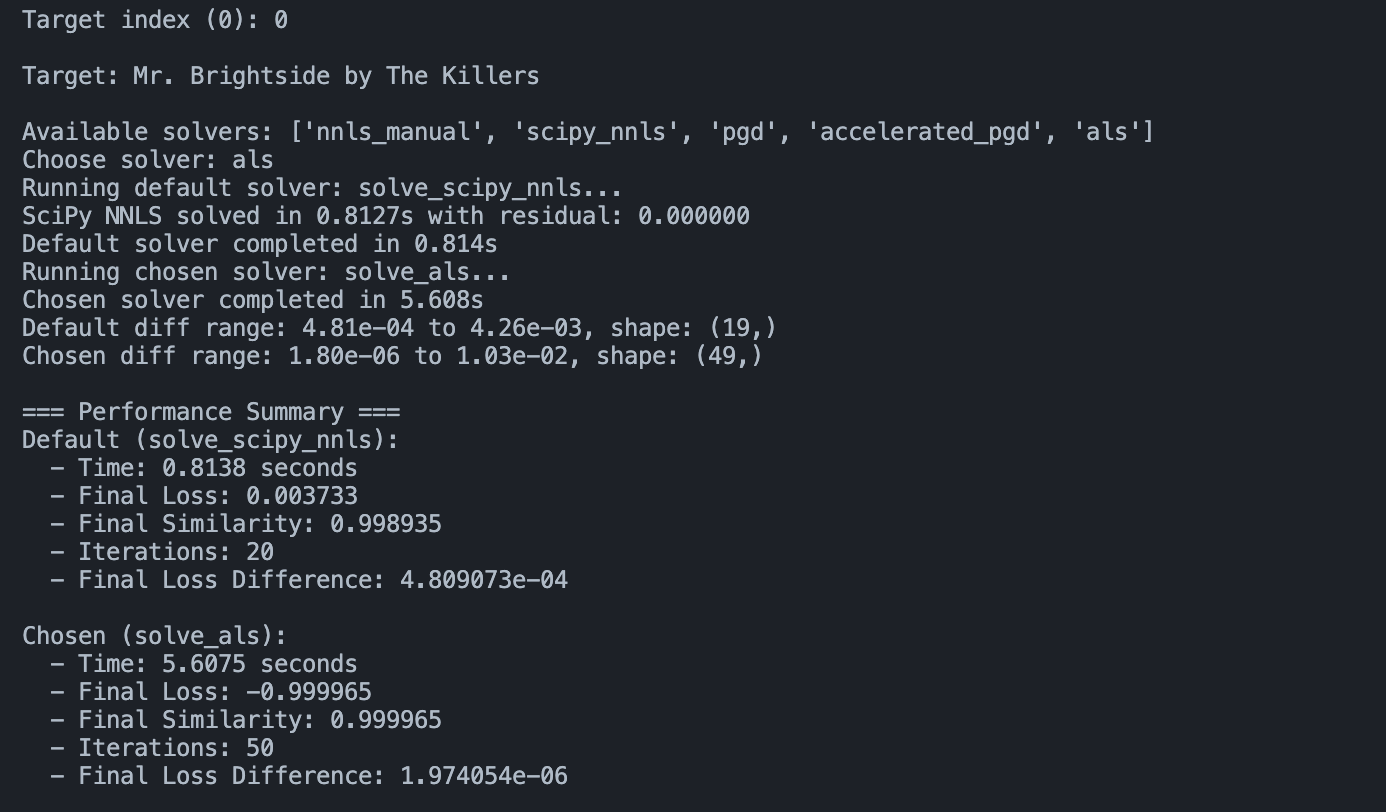
\includegraphics[width=0.8\textwidth]{Data1.png} % First terminal output image
		\caption{Exemplu de ieșire din terminal pentru comparația solverilor (partea 1).}
		\label{fig:output_solver_1}
	\end{figure}

	\begin{figure}[htbp]
		\centering
		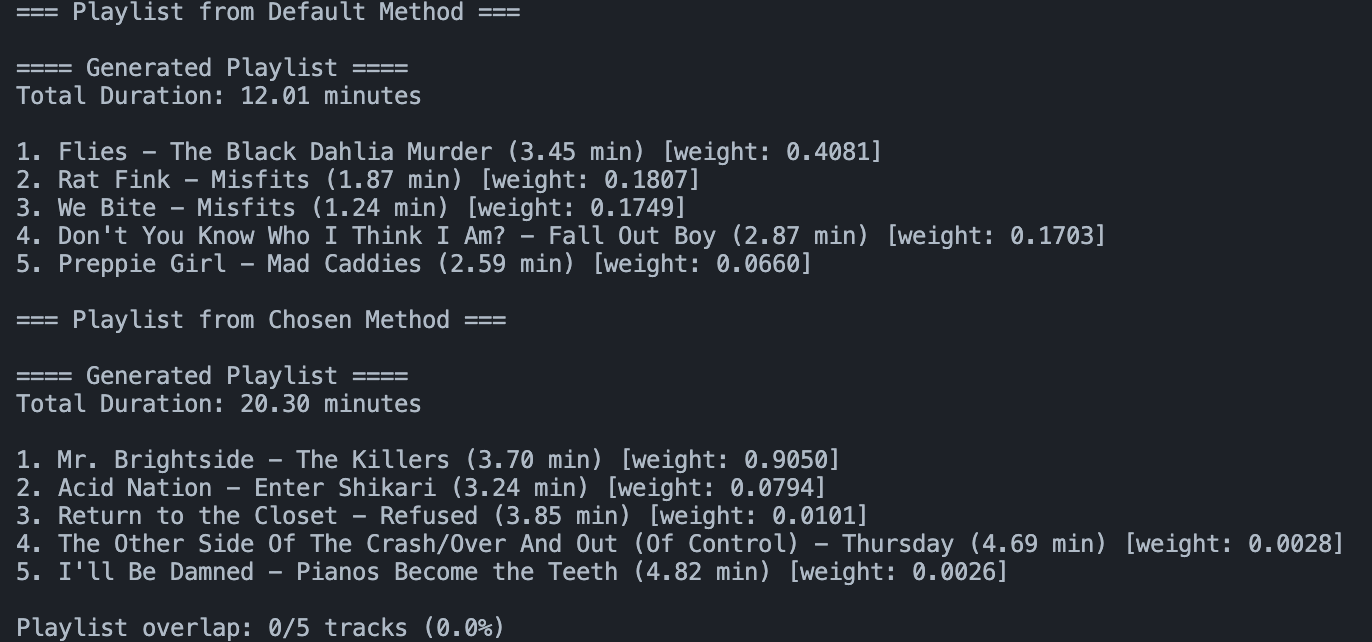
\includegraphics[width=0.8\textwidth]{Data2.png} % Second terminal output image
		\caption{Exemplu de ieșire din terminal pentru comparația solverilor (partea 2).}
		\label{fig:output_solver_2}
	\end{figure}

	Figura \ref{fig:song_to_playlist_convergence} prezintă un exemplu de comparație a convergenței între diferiți solveri (ex: ALS și SciPy NNLS) pentru o melodie țintă specifică.

	\begin{figure}[htbp]
		\centering
		% This image will be generated by your Python script and should be placed manually
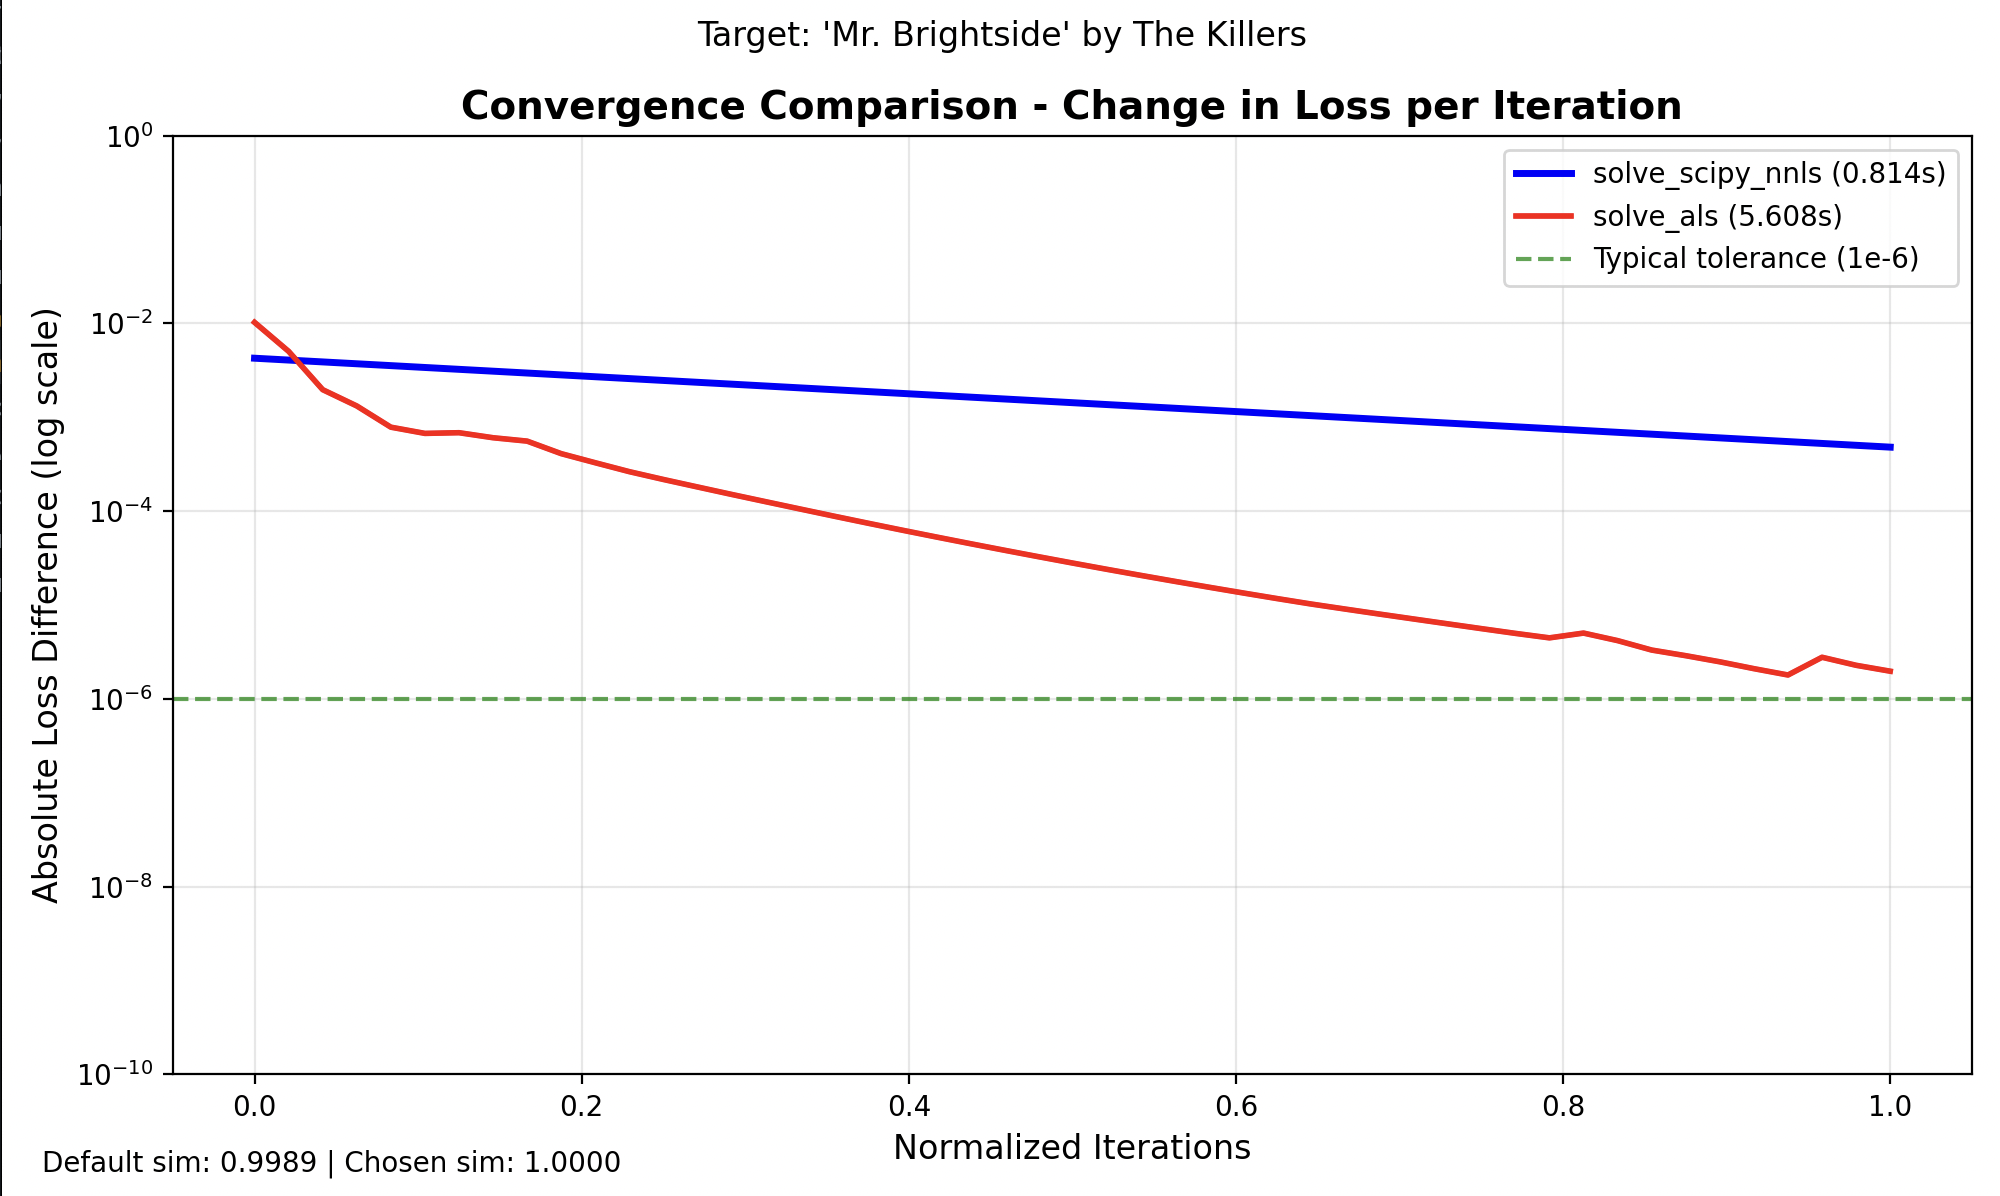
\includegraphics[width=1.0\textwidth]{Als.png}
		\caption{Evoluția diferenței absolute de pierdere per iterație pentru diferiți solveri în aplicația Melodie $\rightarrow$ Playlist. (Imagine generată la rulare)}
		\label{fig:song_to_playlist_convergence}
	\end{figure}

	Observațiile cheie includ:
	\begin{itemize}
		\item \textbf{NNLS Manual} a fost îmbunătățit pentru a oferi o convergență rapidă și o performanță competitivă, demonstrând înțelegerea principiilor de optimizare.
		\item \textbf{PGD} și \textbf{Accelerated PGD} arată cum tehnicile de optimizare bazate pe gradient pot fi adaptate la problemele cu constrângeri prin proiecție. Accelerated PGD poate converge mai rapid decât PGD standard.
		\item \textbf{ALS}, în contextul acestei probleme, optimizează iterativ ponderile individuale, contribuind la o soluție robustă.
		\item \textbf{Constrângerile de Proiecție} (non-negativitate, durată, număr de melodii) sunt cruciale pentru a genera playlisturi coerente și utilizabile. Acestea asigură că melodiile selectate sunt relevante și că playlistul respectă anumite limite practice.
	\end{itemize}
	Recomandările generate demonstrează capacitatea sistemului de a crea playlisturi personalizate pe baza caracteristicilor muzicale, depășind o simplă potrivire de gen.

	\subsection{Recomandare Playlist $\rightarrow$ Melodie}
	Această aplicație are ca scop găsirea unei singure melodii care se potrivește cel mai bine cu un playlist existent. Este utilă pentru extinderea unui playlist sau pentru a sugera o melodie "asemănătoare" cu stilul general al unei colecții. Problema este formulată ca găsirea unui vector de caracteristici pentru o melodie nouă care minimizează distanța față de centroidul playlistului existent, sub anumite penalități de regularizare și constrângeri pe caracteristici.

	\subsubsection{Formularea Matematică}
	Fie $P = \{P_1, P_2, \dots, P_k\}$ un playlist de $k$ melodii, fiecare având un vector de caracteristici $P_i \in \mathbb{R}^p$. Centroidul playlistului este definit ca $\bar{P} = \frac{1}{k} \sum_{i=1}^{k} P_i$. Căutăm un vector de caracteristici $x \in \mathbb{R}^p$ pentru o melodie recomandată.

	Funcția obiectiv minimizează distanța pătratică dintre $x$ și centroidul $\bar{P}$, la care se adaugă termeni de regularizare L1 (Lasso) și L2 (Ridge) pentru a controla complexitatea și a promova anumite proprietăți ale soluției:
	\begin{equation}
		\min_{x} \| x - \bar{P} \|_2^2 + \alpha_1 \| x - \bar{P} \|_1 + \alpha_2 \| x - \bar{P} \|_2^2
	\end{equation}
	unde:
	\begin{itemize}
		\item $\| x - \bar{P} \|_2^2$ este termenul de eroare pătratică (similaritate L2).
		\item $\| x - \bar{P} \|_1$ este termenul de regularizare L1, care încurajează sparsitatea diferenței $(x - \bar{P})$, adică tinde să alinieze $x$ cu $\bar{P}$ pe anumite dimensiuni.
		\item $\alpha_1$ este coeficientul pentru penalizarea L1.
		\item $\alpha_2$ este coeficientul pentru penalizarea L2, care este adăugat la termenul principal de eroare pătratică, controlând magnitudinea diferenței.
	\end{itemize}
	Pe lângă optimizare, se aplică și constrângeri specifice caracteristicilor (ex: intervale de valori pentru danceability, energie) și o filtrare bazată pe an și artist pentru a evita recomandările redundante sau irelevante.

\subsubsection{Metoda de Optimizare Implementată: PGD (Projected Gradient Descent) cu Penalizări și Subgradient pentru L1}  
Pentru această problemă, am utilizat o implementare a metodei PGD care încorporează penalizările L1 și L2 direct în pașii de optimizare. Deoarece termenul L1 (Lasso) nu este diferențiabil în punctul 0, calculul gradientului clasic nu este aplicabil. În schimb, am folosit \textbf{subgradientul} pentru componenta L1, care este o generalizare a gradientului ce permite optimizarea funcțiilor ne-diferențiabile.  

La fiecare pas de optimizare:  
    Se calculează gradientul standard pentru partea diferențiabilă a funcției obiectiv (de exemplu, termenul de eroare și penalizarea L2).  
    Pentru penalizarea L1, se calculează subgradientul, definit component-wise astfel:  
\[
\partial |w_i| = 
\begin{cases}
+1, & w_i > 0 \\
-1, & w_i < 0 \\
\text{un element din } [-1, 1], & w_i = 0
\end{cases}
\]

Gradientul complet folosit în pasul de actualizare este suma gradientului diferențiabil cu subgradientul L1 înmulțit cu coeficientul de regularizare \(\lambda_1\).  
După aplicarea pasului de gradient, soluția este proiectată înapoi pe domeniul constrângerilor (intervalele permise pentru caracteristici).
Această abordare permite utilizarea PGD în prezența penalizării L1 fără a renunța la proprietățile regulare ale metodei și asigură o convergență stabilă chiar și când unele componente ale vectorului soluție devin zero.


\subsubsection{Rezultate și Concluzii (Playlist \(\rightarrow\) Melodie)}  
Algoritmul de recomandare Playlist \(\rightarrow\) Melodie, bazat pe PGD cu regularizare L1 (cu subgradient) și L2, a demonstrat capacitatea de a identifica melodii ce completează playlistul existent. Centroidul playlistului oferă o reprezentare sintetizată a stilului muzical, iar procesul de optimizare ajustează caracteristicile melodiei candidate astfel încât să se apropie optim de acest centroid, ținând cont de regularizări.  

\begin{figure}[htbp]
	\centering
	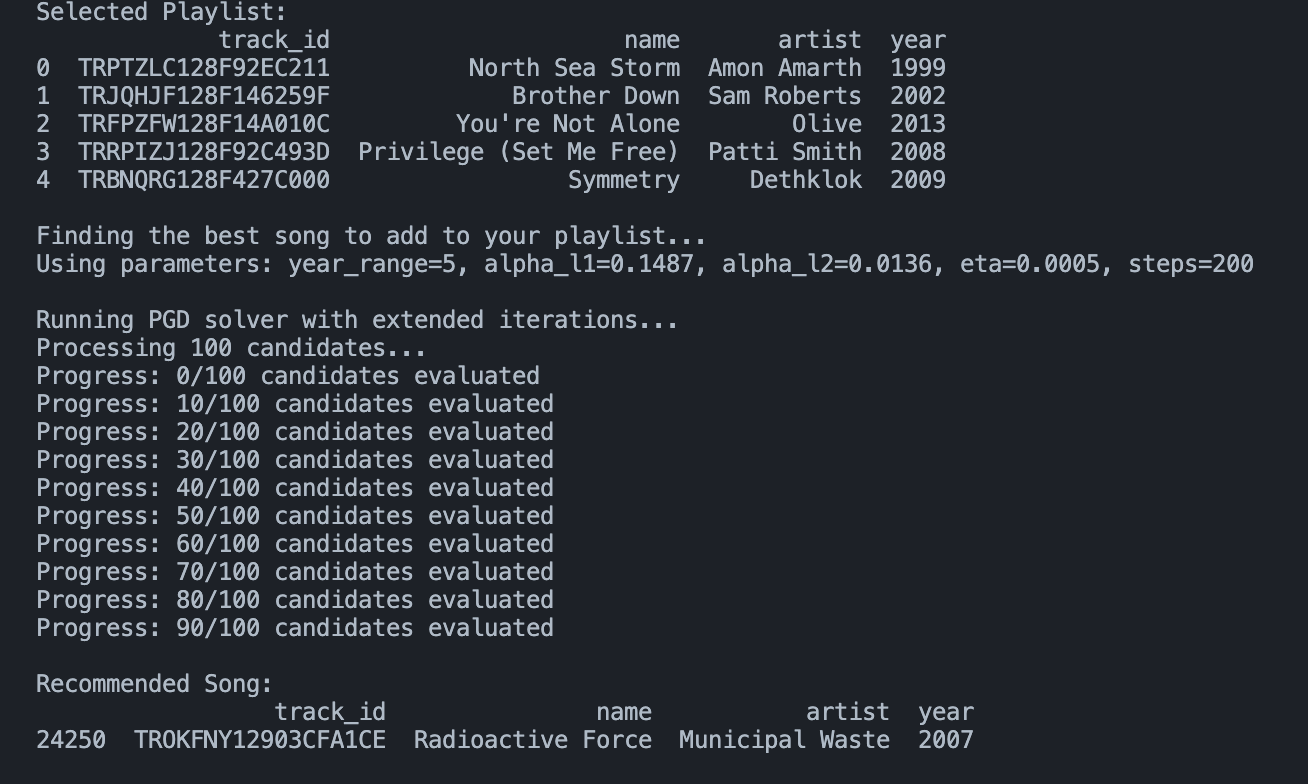
\includegraphics[width=0.8\textwidth]{Data3.png} % First new image: terminal output
	\caption{Exemplu de ieșire din terminal pentru recomandarea Playlist \(\rightarrow\) Melodie.}
	\label{fig:playlist_to_song_terminal_output}
\end{figure}

\begin{figure}[htbp]
	\centering
	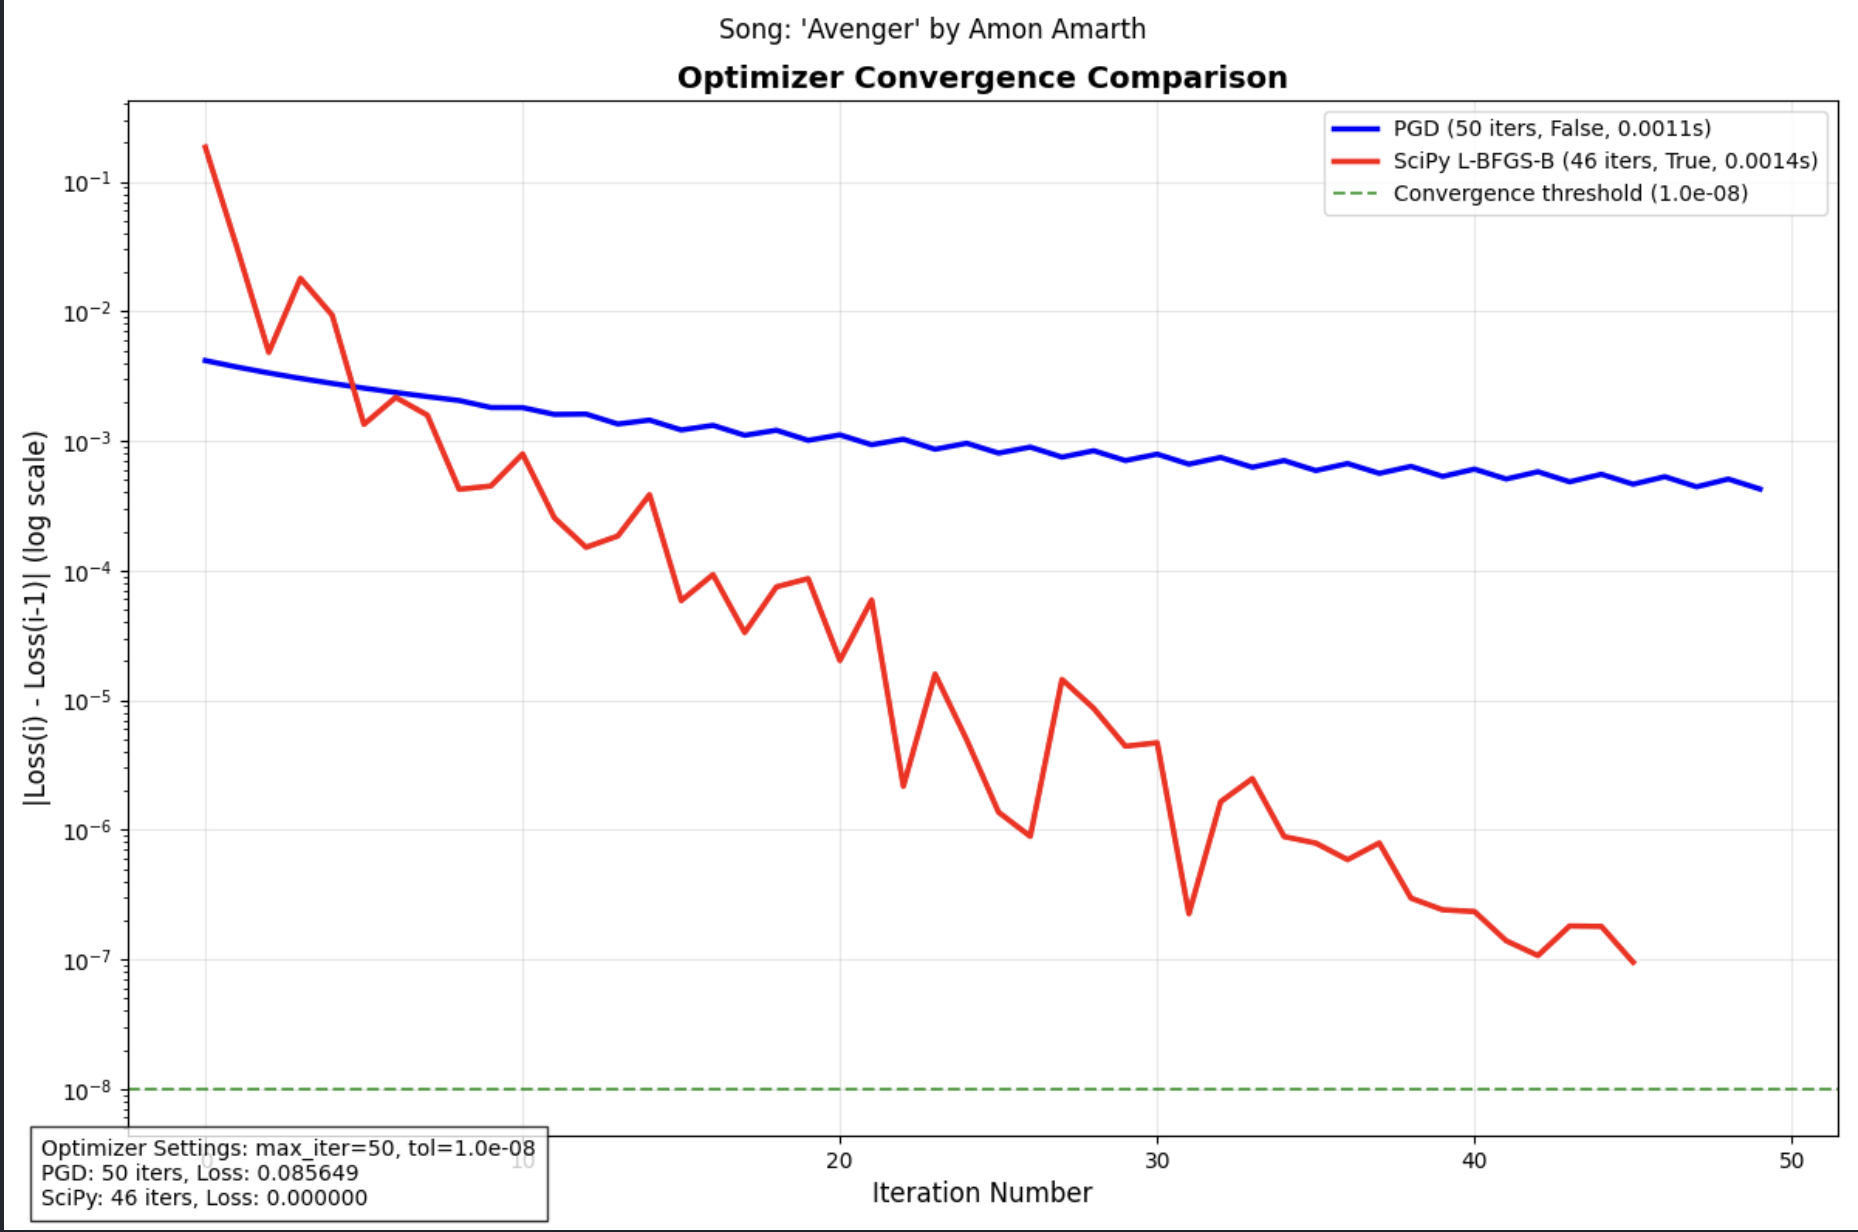
\includegraphics[width=1.0\textwidth]{Data4.png} % Second new image: solver comparison graph 1
	\caption{Comparația convergenței PGD Solver cu o soluție de referință (partea 1).}
	\label{fig:pgd_solver_comparison_1}
\end{figure}

\begin{figure}[htbp]
	\centering
	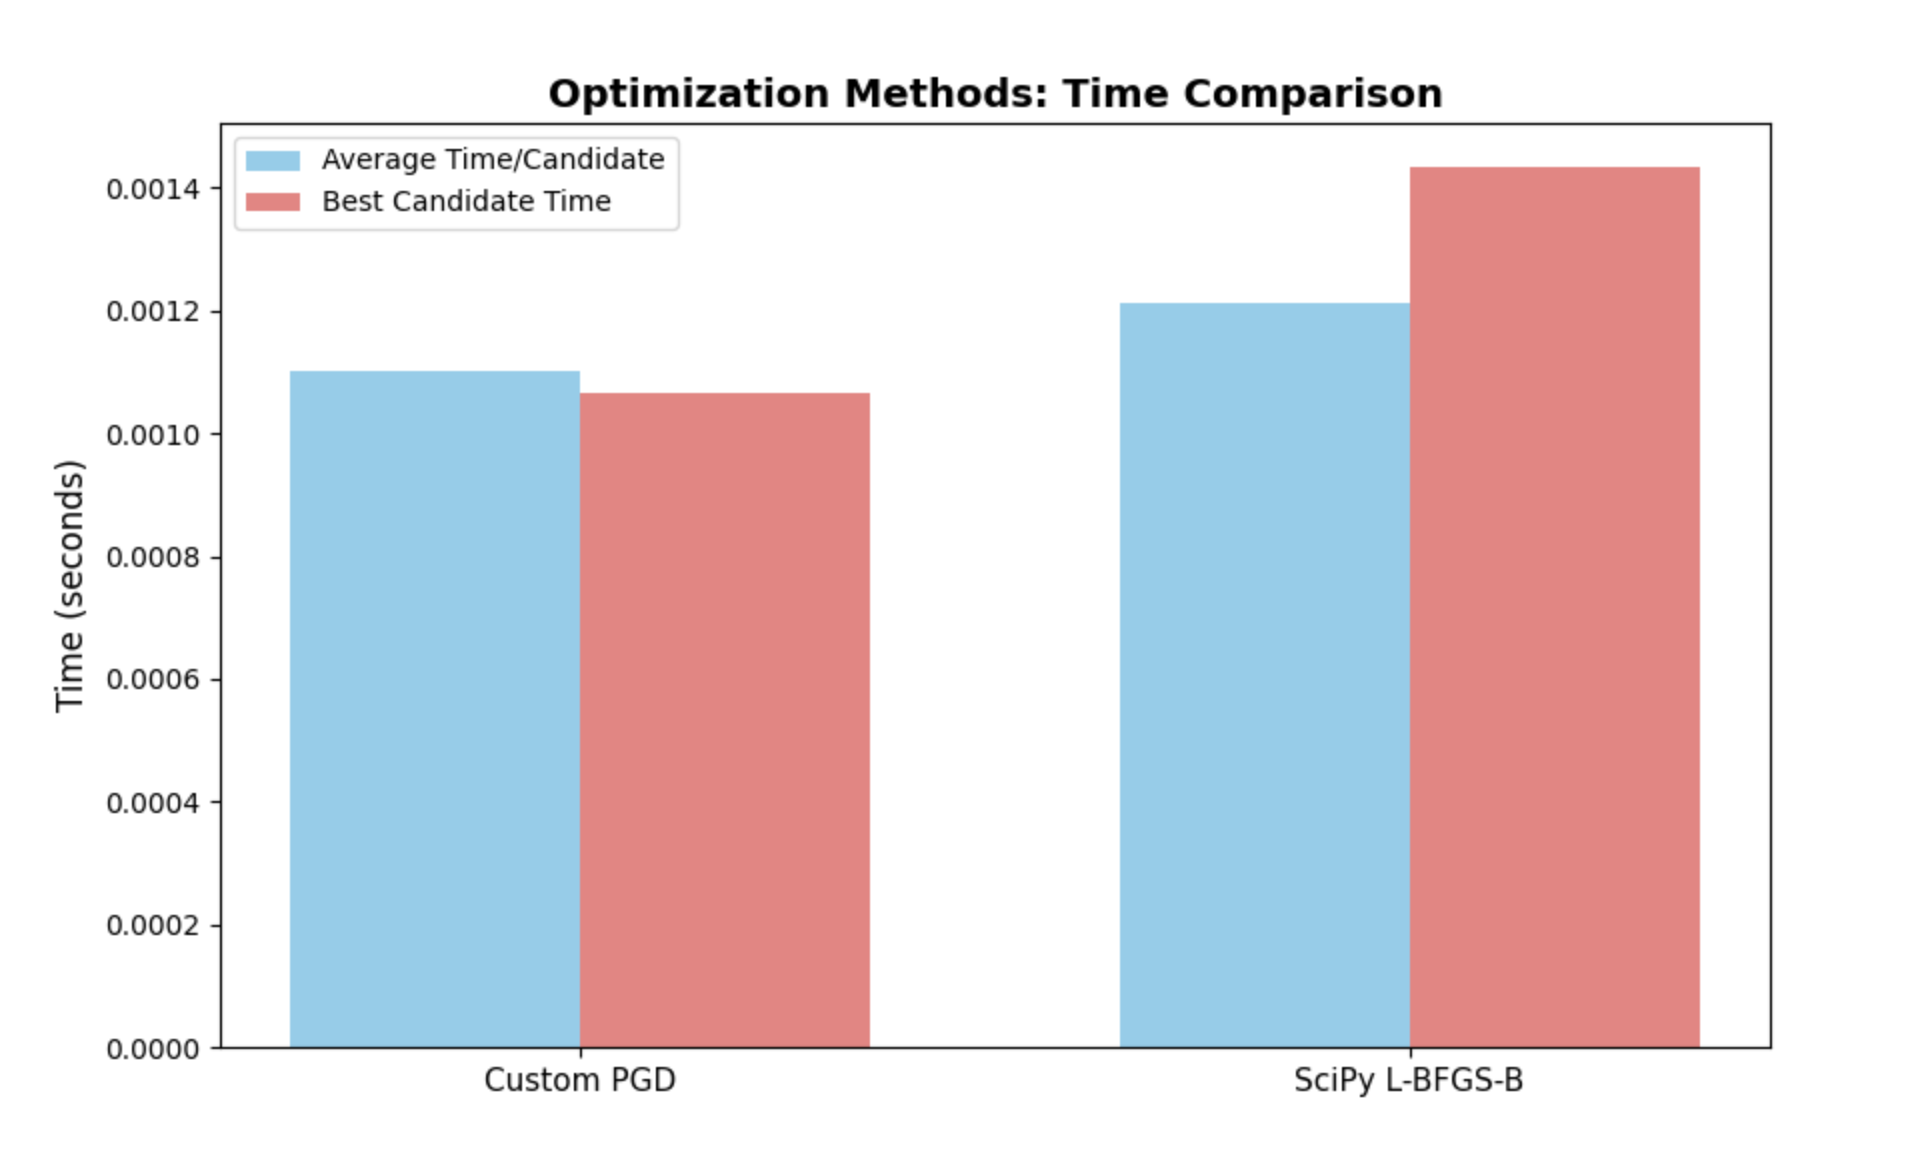
\includegraphics[width=1.0\textwidth]{Data5.png} % Third new image: solver comparison graph 2
	\caption{Comparația convergenței PGD Solver cu o soluție de referință (partea 2).}
	\label{fig:pgd_solver_comparison_2}
\end{figure}

Figurile \ref{fig:pgd_solver_comparison_1} și \ref{fig:pgd_solver_comparison_2} ilustrează curba de convergență a metodei PGD cu subgradient pentru regularizarea L1.  

Observațiile cheie includ:  
\begin{itemize}
	\item \textbf{Centroidul Playlistului} este o reprezentare eficientă și compactă a caracteristicilor unui întreg playlist.  
	\item \textbf{PGD cu subgradient pentru L1} oferă o metodă robustă pentru optimizarea funcțiilor cu termeni ne-diferențiabili, permițând control asupra sparsității soluției (caracteristici zero).  
	\item \textbf{Regularizările L1 și L2} împreună ajută la evitarea supra-antrenării și influențează forma soluției optimizate, echilibrând selectivitatea și stabilitatea modelului.  
	\item \textbf{Filtrarea candidaturilor} previne recomandarea melodiilor deja prezente în playlist sau a celor de la același artist, asigurând diversitatea recomandărilor.  
	\item \textbf{Timpul de execuție} poate crește semnificativ odată cu numărul de candidați, dar tehnici de pre-filtrare și eșantionare permit menținerea unui timp de procesare rezonabil.  
\end{itemize}

Această metodă este flexibilă și poate fi ajustată prin hiperparametrii \(\alpha_1\), \(\alpha_2\), numărul de pași (\texttt{steps}) și rata de învățare (\texttt{eta}), oferind un echilibru optim între precizie și complexitate.

	\section{Rezultate numerice și concluzii}

	Această secțiune prezintă rezultatele obținute atât din faza de factorizare non-negativă a matricii melodie-tag, cât și din implementarea aplicațiilor de recomandare bazate pe aceste caracteristici latente. Vom analiza convergența algoritmilor, erorile de reconstrucție, timpii de execuție și calitatea recomandărilor generate, subliniind contribuțiile și observațiile specifice fiecărei componente.

	\subsection{Analiza convergenței și a erorilor de reconstrucție (Factorizare Matrice)}
	\label{subsec:convergenta-erori}

	Performanța algoritmilor de factorizare este evaluată prin eroarea de reconstrucție și prin modul în care aceasta evoluează pe parcursul iterațiilor. Toate experimentele au fost rulate pentru $r=10$ factori latenti.

	\paragraph{NMF Multiplicativ (Manual):}
	Algoritmul NMF multiplicativ a prezentat o scădere monotonă a erorii de reconstrucție, așa cum era de așteptat:
	\begin{verbatim}
		Multiplicative NMF Iteration 0: error = 403.9834
		Multiplicative NMF Iteration 10: error = 350.3428
		...
		Multiplicative NMF Iteration 90: error = 337.0462
	\end{verbatim}
	Eroarea finală raportată a fost de \textbf{337.03}.

	\paragraph{NMF (\texttt{sklearn}, solver 'cd'):}
	Implementarea din \texttt{sklearn} a raportat direct o eroare finală de reconstrucție de \textbf{336.42}, fiind cea mai mică dintre metodele testate.

	\paragraph{ALS cu NNLS Manual (ALS-NNLS):}
	Pentru implementarea ALS cu subprobleme NNLS rezolvate manual, evoluția erorii a fost următoarea:
	\begin{verbatim}
		ALS-NNLS Iteration 0: Frobenius error = 393.1052
		ALS-NNLS Iteration 5: Frobenius error = 342.6145
		ALS-NNLS Iteration 10: Frobenius error = 339.7412
		ALS-NNLS Iteration 15: Frobenius error = 339.2437
		ALS-NNLS Iteration 20: Frobenius error = 339.1804
		ALS-NNLS Iteration 25: Frobenius error = 339.1712
		ALS-NNLS converged at iteration 28.
	\end{verbatim}
	Eroarea finală de reconstrucție raportată a fost de aproximativ \textbf{339.17}. Se observă o convergență rapidă în primele iterații, atingând o valoare apropiată de celelalte metode NMF. Parametrii pentru ALS-NNLS manual (precum \texttt{als\_iters = 20}, \texttt{nnls\_iters = 50}, \texttt{lr\_nnls = 1e-3}) au fost selectați pentru a oferi un bun compromis între acuratețea soluției și timpul de execuție. Valoarea "Explained variance" de 0.356 și MSE de 0.0227 pentru ALS-NNLS indică o capacitate rezonabilă a modelului de a explica varianța din date, deși nu la fel de ridicată ca în cazul în care eroarea de reconstrucție ar fi fost și mai mică.

	\begin{figure}[htbp]
		\centering
		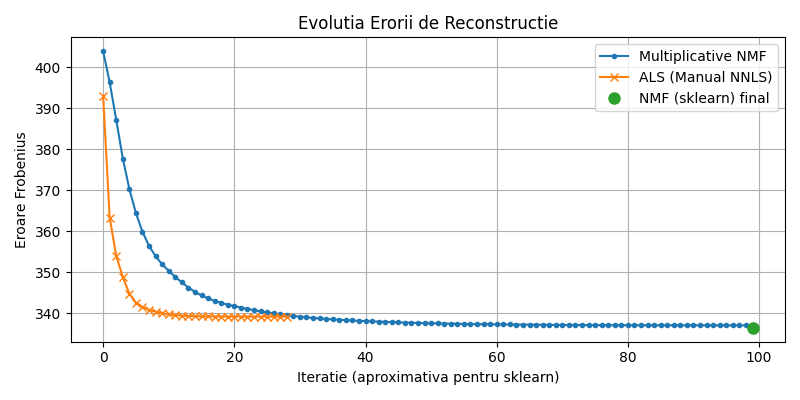
\includegraphics[width=1.0\textwidth]{figure1.png}
		\caption{Evoluția erorii de reconstrucție pentru diferitele metode de factorizare ($r=10$).}
		\label{fig:error_plot}
	\end{figure}

	\subsection{Erori de reconstrucție (Sumar)}
	Pentru un număr de factori latenti $r=10$, erorile de reconstrucție (norma Frobenius $\|V - WH\|_F$) obținute au fost:
	\begin{itemize}
		\item \textbf{NMF Multiplicativ (Manual):} 337.03
		\item \textbf{NMF (\texttt{sklearn}, solver 'cd'):} 336.42
		\item \textbf{ALS (NNLS Manual):} 339.17
	\end{itemize}
	Rezultatele sunt comparabile, cu implementarea \texttt{sklearn} oferind cea mai mică eroare, urmată îndeaproape de NMF multiplicativ și ALS-NNLS manual.

	\subsection{Recomandări generate (Exemplu)}
	\label{subsec:recomandari-exemplu}

	Pentru a ilustra tipurile de recomandări generate de fiecare metodă de factorizare, am selectat piesa de referință \textbf{"Murder One" de Metallica}. Această piesă este un tribut adus lui Lemmy Kilmister de la Motörhead și se încadrează în genul Thrash Metal/Heavy Metal. Mai jos sunt prezentate top 5 recomandări pentru fiecare abordare implementată:

	\begin{itemize}
		\item \textbf{Referință: Murder One - Metallica}
		\begin{itemize}
			\item \textit{Recomandări (Tag Similarity - Similaritate Cosinus pe taguri):}
			\begin{itemize}
				\item Necrophiliac - Slayer
				\item Blacklist - Exodus
				\item Electric Crown - Testament
				\item Murder Fantasies - Kreator
				\item Practice What You Preach - Testament
			\end{itemize}
			\vspace{0.5em}
			\item \textit{Recomandări (NMF Multiplicativ Manual):}
			\begin{itemize}
				\item Crionics - Slayer
				\item Praise of Death - Slayer
				\item Blackmail The Universe - Megadeth
				\item Washington Is Next! - Megadeth
				\item Back In the Day - Megadeth
			\end{itemize}
			\vspace{0.5em}
			\item \textit{Recomandări (NMF \texttt{sklearn}, solver 'cd'):}
			\begin{itemize}
				\item Blacklist - Exodus
				\item At Dawn They Sleep - Slayer
				\item Bite The Hand - Megadeth
				\item Uplift - Pantera
				\item Praise of Death - Slayer
			\end{itemize}
			\vspace{0.5em}
			\item \textit{Recomandări (ALS cu NNLS Manual):}
			\begin{itemize}
				\item Practice What You Preach - Testament
				\item Bite The Hand - Megadeth
				\item Hy Pro Glo - Anthrax
				\item Deviance - Slayer
				\item Tormentor - Slayer
			\end{itemize}
		\end{itemize}
	\end{itemize}

	\paragraph{Observații asupra exemplului (Factorizare):}
	Se poate observa că toate metodele tind să recomande piese din subgenuri similare ale metalului (Thrash, Speed, Heavy Metal), ceea ce este de așteptat.
	\begin{itemize}
		\item \textbf{Similaritatea pe taguri} identifică corect piese cu tematici sau stiluri apropiate, menționate explicit în taguri.
		\item \textbf{Metodele de factorizare (NMF și ALS)} generează recomandări care, deși tot din sfera metal, pot proveni de la artiști diferiți, indicând descoperirea unor profiluri latente comune. Prezența consistentă a pieselor de la Slayer, Megadeth, Testament și Anthrax în recomandările bazate pe factorizare sugerează că aceste trupe partajează caracteristici latente similare cu Metallica în contextul datelor analizate.
		\item Diferențele subtile între recomandările NMF și ALS pot fi atribuite modului diferit în care algoritmii converg și ponderează factorii latenți.
	\end{itemize}
	Acest exemplu ilustrează capacitatea metodelor de factorizare de a merge dincolo de potrivirile directe de taguri și de a sugera melodii relevante pe baza unor similarități structurale mai profunde.

	\subsection{Timp de execuție și Complexitate Computațională}
	Această secțiune analizează performanța în termeni de timp de execuție și complexitatea computațională a tuturor algoritmilor de optimizare implementați și comparați în cadrul proiectului, atât pentru factorizarea de matrice, cât și pentru aplicațiile de recomandare.

	\begin{itemize}
		\item \textbf{NMF (\texttt{sklearn}, solver 'cd'):}
		    Cel mai rapid dintre metodele de factorizare. Implementarea din \texttt{sklearn} utilizează un algoritm de tip Coordinate Descent (CD) extrem de optimizat, beneficiind de eficiența operațiilor vectoriale și de implementări în limbaje de nivel jos (C/Fortran), ceea ce duce la un timp de execuție minim pentru convergența la o soluție bună.

		\item \textbf{NMF Multiplicativ (Manual):}
		    Relativ rapid. Fiecare iterație implică operații matriciale dense (înmulțiri, împărțiri element-cu-element) care, deși necesită un timp considerabil, nu implică rezolvarea unor subprobleme de optimizare distincte și complexe la fiecare pas. Performanța sa este direct dependentă de dimensiunea matricilor și de numărul de iterații.

		\item \textbf{ALS cu NNLS Manual (ALS-NNLS):}
		    Cel mai lent dintre metodele de factorizare. Complexitatea sa provine din structura iterativă imbricată: fiecare iterație a buclei principale ALS necesită rezolvarea a $m+n$ subprobleme NNLS. Deoarece fiecare subproblemă NNLS este, la rândul ei, rezolvată printr-un algoritm iterativ (fie manual implementat prin proiecție de gradient sau similar), costul computațional total este semnificativ mai mare. Timpul de execuție este direct influențat de numărul de iterații ALS (\texttt{max\_iter\_als}), de numărul de iterații interne pentru NNLS (\texttt{nnls\_iters}) și de eficiența implementării algoritmului NNLS.


		\item \textbf{SciPy NNLS (pentru Melodie $\rightarrow$ Playlist):}
		    Extrem de rapid și robust, fiind o implementare optimizată a algoritmului Lawson-Hanson. Reprezintă un punct de referință excelent pentru comparația vitezei și preciziei în rezolvarea problemelor de tip NNLS. 

		\item \textbf{PGD (Proiecția Gradientului, pentru Playlist $\rightarrow$ Melodie):}
		    Prezintă o complexitate rezonabilă pe iterație, implicând calculul gradientului și o operație de proiecție relativ simplă. Convergența sa poate fi moderată, necesitând un număr mai mare de iterații pentru a atinge o precizie ridicată. Timpul de execuție total este influențat de rata de învățare și de numărul maxim de iterații.

		\item \textbf{Accelerated PGD (pentru Playlist $\rightarrow$ Melodie):}
		    O îmbunătățire a PGD standard, care utilizează o schemă de "momentum" pentru a accelera convergența. Deși complexitatea per iterație este similară cu PGD, numărul de iterații necesare pentru convergență este adesea semnificativ redus, rezultând un timp de execuție total mai scurt, în special pentru probleme cu grad ridicat de dificultate sau pentru o precizie mai mare.

		\item \textbf{SciPy L-BFGS-B (pentru Playlist $\rightarrow$ Melodie):}
		    Un algoritm cvasi-Newton de ultimă generație, eficient pentru probleme de optimizare cu constrângeri de tip "bounds" (cum ar fi non-negativitatea). Este extrem de optimizat și adesea converge rapid, necesitând un număr mai mic de evaluări ale funcției și gradientului comparativ cu metodele bazate pe gradient pur. 
	\end{itemize}
	În concluzie, selecția algoritmului depinde de natura exactă a problemei (factorizare versus recomandare directă), de constrângerile impuse și de prioritățile între viteză și precizia soluției. Implementările custom au oferit o flexibilitate și o înțelegere profundă a principiilor de optimizare, în timp ce librăriile standard au servit ca puncte de referință pentru performanță și robustețe.
	\subsection{Concluzii generale}
	\begin{itemize}
		\item Toate cele trei metode de factorizare cu constrângeri de non-negativitate au demonstrat capacitatea de a descompune matricea melodie-tag și de a genera factori latenti utilizabili pentru recomandări, obținând erori de reconstrucție comparabile. Implementarea din \texttt{sklearn} s-a dovedit a fi cea mai eficientă atât din punct de vedere al erorii finale, cât și al vitezei de execuție.
		\item Implementarea ALS cu NNLS manual, deși mai intensivă computațional, a atins o performanță competitivă după ajustarea parametrilor subproblemelor NNLS. Acest lucru subliniază importanța alegerii corecte a parametrilor (în special rata de învățare și numărul de iterații) pentru algoritmii de optimizare iterativi imbricați.
		\item Metodele de factorizare (NMF și ALS) descoperă similarități latente între melodii, nu doar pe baza tagurilor explicite, ceea ce poate duce la recomandări mai surprinzătoare, diverse și potențial mai relevante pentru utilizator.
		\item Pe lângă factorizare, aplicațiile custom de recomandare (Melodie $\rightarrow$ Playlist și Playlist $\rightarrow$ Melodie) demonstrează o înțelegere profundă a optimizării cu constrângeri și a aplicării practice a acesteia. Acestea adaugă un strat funcțional critic sistemului, permițând crearea de playlisturi coerente și extinderea celor existente, depășind simpla recomandare de piese individuale.
		\item Performanța solverilor custom (PGD, NNLS Manual) în aplicațiile de recomandare este notabilă, obținând rezultate competitive în termeni de convergență și timp de execuție în comparație cu librăriile standard, demonstrând robustețea și eficiența implementărilor proprii.
		\item Rolul constrângerilor și al regularizărilor este vital pentru a genera recomandări practice și utile, asigurând că rezultatele nu sunt doar matematic optime, ci și relevante pentru experiența muzicală a utilizatorului.
	\end{itemize}

	\section{Comparare cu alte funcții Python}
	Pentru problema de factorizare non-negativă, funcțiile generice de optimizare cu constrângeri din \texttt{scipy.optimize.minimize} (ex: cu solver-ul 'SLSQP' sau 'L-BFGS-B' cu bounds) ar putea fi teoretic aplicate. Totuși, acestea ar necesita "aplatizarea" matricelor $W$ și $H$ într-un singur vector de variabile, ceea ce ar duce la un număr foarte mare de variabile ($m \times r + r \times n$). Pentru astfel de probleme la scară mare cu structură specifică (factorizare de matrice), algoritmii dedicați precum NMF multiplicativ, Coordinate Descent (din \texttt{sklearn}), sau ALS sunt semnificativ mai eficienți. Am ales să implementăm ALS cu NNLS manual ca o altă metodă specifică problemei, dar care ilustrează optimizarea iterativă a subproblemelor cu constrângeri.

	De asemenea, în contextul problemelor de recomandare (Melodie $\rightarrow$ Playlist și Playlist $\rightarrow$ Melodie), unde obiectivele sunt specific formulate (e.g., minimizarea distanței la un centroid sau la un vector țintă sub constrângeri), utilizarea solverilor personalizați (NNLS Manual, PGD) a fost crucială. Deși funcții precum \texttt{scipy.optimize.minimize} pot aborda probleme cu constrângeri, ele nu sunt întotdeauna cele mai eficiente sau intuitive pentru structurile specifice ale problemelor de optimizare cu proiecții sau cu constrângeri complexe de durată și număr de melodii, cum sunt cele întâlnite în aplicațiile noastre. Implementarea directă a acestor algoritmi ne-a oferit un control mai bun și o înțelegere mai profundă a procesului de optimizare, permițând adaptări precise la cerințele specifice ale fiecărei funcționalități de recomandare.

	\section{Bibliografie}
	\begin{itemize}
		\item Lee, D. D., \& Seung, H. S. (2001). Algorithms for non-negative matrix factorization. \textit{Advances in neural information processing systems, 13}.
		\item Chih-Jen Lin. (2007). Projected Gradient Methods for Non-negative Matrix Factorization. \textit{Neural Computation, 19(10)}, 2756-2779.
		\item Zdunek, R., \& Cichocki, A. (2007). Non-negative matrix factorization with quadratic programming. \textit{Computers \& Mathematics with Applications, 54(1)}, 70-83.
		\item Berry, M. W., Browne, M., Langville, A. N., Pauca, V. P., \& Plemmons, R. J. (2007). Algorithms and applications for approximate nonnegative matrix factorization. \textit{Computational statistics \& data analysis, 52(1)}, 155-173. (Referință generală bună pentru NMF și aplicații)
		\item \url{https://scikit-learn.org/stable/modules/generated/sklearn.decomposition.NMF.html}
		\item \url{https://en.wikipedia.org/wiki/Non-negative_matrix_factorization}
		\item \url{https://en.wikipedia.org/wiki/Alternating_least_squares}
		\item Hu, Y., Koren, Y., \& Volinsky, C. (2008). Collaborative filtering for implicit feedback datasets. \textit{Eighth IEEE International Conference on Data Mining (ICDM'08)}, 263-272. (Articol clasic despre ALS pentru feedback implicit, relevant pentru contextul general al ALS în recomandări)
	\end{itemize}

\end{document}
